\documentclass{standalone}
\usepackage{tikz}

\begin{document}
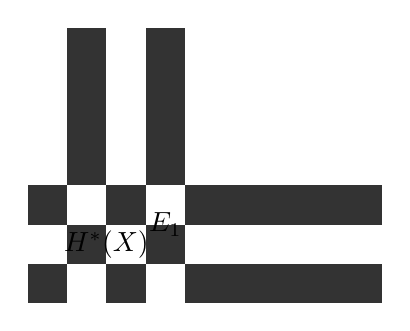
\begin{tikzpicture}[scale=0.5]
    % Define colors for alternating squares
    \colorlet{squareColorA}{black!80}
    \colorlet{squareColorB}{white}

    % Draw the grid of squares
    \foreach \x in {0,...,4} {
        \foreach \y in {0,...,3} {
            \ifodd\x
                \ifodd\y
                    \fill[squareColorA] (\x,\y) rectangle+(\x+1,\y+1);
                \else
                    \fill[squareColorB] (\x,\y) rectangle+(\x+1,\y+1);
                \fi
            \else
                \ifodd\y
                    \fill[squareColorB] (\x,\y) rectangle+(\x+1,\y+1);
                \else
                    \fill[squareColorA] (\x,\y) rectangle+(\x+1,\y+1);
                \fi
            \fi
        }
    }

    % Add labels if needed
    \node at (2,1.5) {$H^*(X)$};
    \node at (3.5,2) {$E_1$};
\end{tikzpicture}
\end{document}